

%\begin{document}
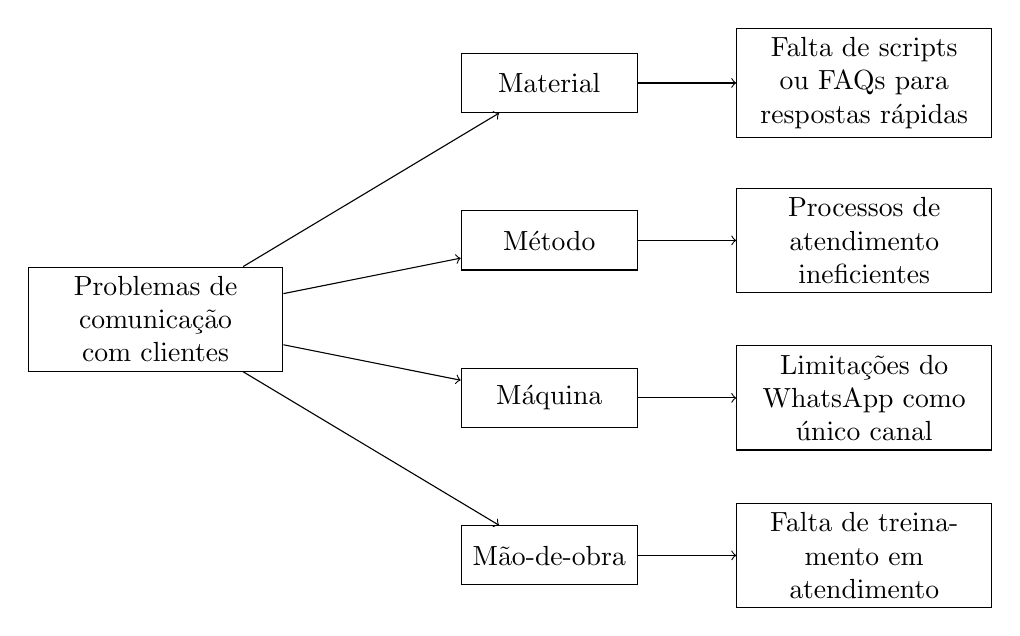
\begin{tikzpicture}[
    node distance=2cm,
    problema/.style={rectangle, draw, fill=white, text width=3cm, text centered, minimum height=1cm},
    categoria/.style={rectangle, draw, fill=white, text width=2cm, text centered, minimum height=0.75cm},
    causa/.style={rectangle, draw, fill=white, text width=3cm, text centered, minimum height=0.75cm}
]

% Problema central
\node[problema] (problema) {Problemas de comunicação com clientes};

% Categorias principais
\node[categoria] (material) at (5,3) {Material};
\node[categoria] (metodo) at (5,1) {Método};
\node[categoria] (maquina) at (5,-1) {Máquina};
\node[categoria] (mao) at (5,-3) {Mão-de-obra};

% Causas específicas
\node[causa] (causa1) at (9,3) {Falta de scripts ou FAQs para respostas rápidas};
\node[causa] (causa2) at (9,1) {Processos de atendimento ineficientes};
\node[causa] (causa3) at (9,-1) {Limitações do WhatsApp como único canal};
\node[causa] (causa4) at (9,-3) {Falta de treinamento em atendimento};

% Conexões
\draw[->] (problema) -- (material);
\draw[->] (problema) -- (metodo);
\draw[->] (problema) -- (maquina);
\draw[->] (problema) -- (mao);

\draw[->] (material) -- (causa1);
\draw[->] (metodo) -- (causa2);
\draw[->] (maquina) -- (causa3);
\draw[->] (mao) -- (causa4);

\end{tikzpicture}
%\end{document}